\documentclass[11pt]{article}
% Adapted from an original template by Hlyni Arnórssyni,
% Reykjavik University, Iceland

% ------------------------------ PAGE SETTINGS ------------------------------
\usepackage{geometry}

\geometry{
    paper=a4paper,
    top=2.5cm,
    bottom=2.5cm,
    left=2.5cm,
    right=2.4cm,
    headheight=0.75cm,
    footskip=1.5cm,
    headsep=0.75cm
}

% ------------------------------ BASIC PACKAGES ------------------------------
\usepackage{blindtext}

% Character encoding
\usepackage[T1]{fontenc}
\usepackage[utf8]{inputenc}

% Mathematics
\usepackage{amsmath, amsfonts, amsthm, amssymb}
\usepackage{braket, nicefrac}

% SI units
\usepackage{siunitx}

% Lists / columns
\usepackage{enumitem, multicol}

% ------------------------------ FIGURES ------------------------------
\usepackage{graphicx}
\usepackage{float}
\usepackage{keystroke}
\usepackage{pgfplots}
\usepgfplotslibrary{units}
\pgfplotsset{compat=1.16}

% Search these locations automatically for figures
\graphicspath{{fig/}{graphics/}{Graphics/}{./}}

% ------------------------------ TABLES ------------------------------
\usepackage{tabularx}
\usepackage{array}
\usepackage[table]{xcolor}

% ------------------------------ TYPOGRAPHY ------------------------------
\usepackage{caption}
\usepackage{titlesec}
\usepackage{microtype}
\usepackage{csquotes}

% ------------------------------ COLORS ------------------------------
\definecolor{GWBlue}{HTML}{1E4E79}

% ------------------------------ SECTION STYLING ------------------------------
\titleformat{\section}
  {\Large\bfseries\color{GWBlue}}
  {\thesection.}
  {0.40em}
  {}

\titlespacing*{\section}
  {0pt}
  {0.70em}
  {0.28em}

% ------------------------------ CAPTION STYLING ------------------------------
\captionsetup{
    font=small,
    labelfont=bf,
    textfont=it,
    labelsep=period,
    skip=4pt
}

% ------------------------------ PARAGRAPH SPACING ------------------------------
\setlength{\parindent}{0pt}
\setlength{\parskip}{0.30em}

% ------------------------------ BIBLIOGRAPHY ------------------------------
\usepackage[
    backend=biber,
    style=authoryear,
    sorting=none,
    giveninits=true,
    maxbibnames=99,
    dashed=false
]{biblatex}

\addbibresource{references.bib}

\DeclareNameAlias{sortname}{family-given}
\DeclareNameAlias{default}{family-given}
\DeclareFieldFormat[article]{title}{#1}
\DeclareFieldFormat[misc]{title}{#1}
\renewbibmacro{in:}{}

\AtEveryBibitem{%
    \clearfield{doi}%
    \clearfield{urldate}%
}

\AtBeginBibliography{\small}
\setlength{\bibitemsep}{0.35em}

% ------------------------------ HYPERLINKS ------------------------------
\usepackage{hyperref}

\hypersetup{
    colorlinks=true,
    linkcolor=GWBlue,
    citecolor=GWBlue,
    urlcolor=GWBlue
}
\setlength{\emergencystretch}{3em}

\begin{document}

\begin{titlepage}
\centering
\thispagestyle{empty}

\vspace*{0.15in}


\includegraphics[
    width=0.5\textwidth
]{gwu_logo.pdf}

\vspace{0.28in}

{\large\bfseries Data Science Program\par}
{\large\bfseries Department of Data Science\par}
{\large DATS 6501 - Capstone Project - Fall 2026\par}

\vspace{0.38in}

{\Large\bfseries
Post-Training Analysis \& Novelty Detection Using\par}

\vspace{0.08in}

{\Large\bfseries
Neural Network Self-Organizing Maps (NNSOM)\par}

\vspace{0.34in}

{\large\bfseries
PHASE 2 REPORT\par}

\vspace{0.22in}

{\large\bfseries
NNSOM Training, Cluster and Error Analysis\par}

\vspace{0.36in}

{\large\bfseries Capstone - Group 5\par}

\vspace{0.08in}

{\large\bfseries Fyrooz Anika Khan\par}
{\large\bfseries Nazish Atta\par}

\vspace{0.30in}

{\large The George Washington University\par}
{\large Washington, DC\par}

\vspace{0.30in}

{\large\itshape Supervised by\par}
{\large\itshape Dr. Amir Jafari\par}
{\large\itshape Associate Professor of Data Science\par}

\vspace*{\fill}

\end{titlepage}

\section{SOM 15$\times$15 Overview}

This phase applies a 15$\times$15 Self-Organizing Map (SOM) to the
84-dimensional \texttt{fc2} representations extracted from the pretrained
MNIST CNN. The SOM was trained with seed 42 on 49,000 training embeddings and
validated on 10,500 held-out validation embeddings. The objective is to examine
whether topology-preserving organization of the learned representation reveals
class structure, density patterns, and localized validation weaknesses
\cite{kohonen1990som,jafari_nnsom}.

\textbf{Summary of the results.}
\begin{itemize}[leftmargin=1.4em, itemsep=1pt]
  \item \textbf{The map trained well.} Every one of the 225 cells is used, the training error settles after a sharp early drop, and training and validation images fit the map equally well (quantization error 1.039 and 1.041), so the map is not over-fitted to the training images.
  \item \textbf{The digits form clean regions.} 98.2\% of the validation images sit in a cell whose most common digit is their own digit. With shuffled labels this would be only 17.4\%.
  \item \textbf{The CNN's mistakes gather in a few cells.} Eleven ``hotspot'' cells (5\% of the map) hold about 11 times their fair share of the mistakes, tested on images not used to pick them. The mistakes sit where digits mix, such as 4 and 9 or 5 and 0. The same holds on 10$\times$10 and 20$\times$20 maps.
  \item \textbf{The pattern is real, but the SOM is not the best mistake finder.} A k-means grouping finds mistakes about as well as the SOM cells, and the CNN's own confidence finds them much better. The SOM's value is the picture it gives of \emph{where} the mistakes are.
\end{itemize}

\subsection*{Where each item of the plan is covered}

{\small
\renewcommand{\arraystretch}{1.12}
\begin{tabularx}{\textwidth}{|>{\raggedright\arraybackslash}p{0.52\textwidth}|X|}
\hline
\textbf{What Phase 2 asks for} & \textbf{Where} \\ \hline
Set up NNSOM, choose grid size and training settings (grid comparison, Optuna check) & Section~\ref{sec:training}, Table~\ref{tab:grids}, Figure~\ref{fig:gridcmp} \\ \hline
Train on training embeddings, monitor quantization error per epoch & Figure~\ref{fig:qe} \\ \hline
Component planes, hit histogram, U-matrix & Figures~\ref{fig:umatrix} and~\ref{fig:planes} \\ \hline
Assign each image to its best-matching cell; colour the map by digit & Section~\ref{sec:cluster}, Figure~\ref{fig:classmap} \\ \hline
Cluster purity and class--cell intersection & Section~\ref{sec:cluster}, Figure~\ref{fig:classmap} \\ \hline
Confusion heatmaps overlaid on the map & Figure~\ref{fig:overlay} \\ \hline
Correct against misclassified images on the map; error hotspots & Section~\ref{sec:error}, Table~\ref{tab:hotspots}, Figure~\ref{fig:errormaps} \\ \hline
Images in the hotspots, and why they are hard & Figure~\ref{fig:samples}, Section~\ref{sec:error} \\ \hline
\end{tabularx}}

\section{Key terms in plain words}

{\small
\renewcommand{\arraystretch}{1.12}
\begin{tabularx}{\textwidth}{|>{\raggedright\arraybackslash}p{0.24\textwidth}|X|}
\hline
\textbf{Term} & \textbf{What it means} \\ \hline
Embedding (fc2) & The 84 numbers the CNN computes for an image just before it gives its answer. The SOM is trained on these numbers, not on the pixels. \\ \hline
SOM, cell (neuron) & A grid of cells, each holding a weight vector of 84 numbers. After training, similar images land in the same or nearby cells. \\ \hline
Best-matching unit (BMU) & The cell whose weights are closest to an image's embedding. Every image is assigned to its BMU. \\ \hline
Neighbourhood radius & How far on the grid the winning cell's ``pull'' reaches during training. It starts large (so the map orders itself) and shrinks to 1 (so it fits the data). \\ \hline
Quantization error (QE) & The average distance between an image and its BMU. Lower means the map fits the data more closely. \\ \hline
Topological error (TE1) & The share of images whose two closest cells are not next to each other on the grid. Lower means a better ordered map. \\ \hline
Hit histogram & How many images land in each cell. \\ \hline
U-matrix & The distance between each cell and its neighbours. High values (dark red) mark borders between groups of similar cells. \\ \hline
Component plane & One map per embedding number, showing where on the grid that number is high or low. \\ \hline
Purity, entropy & Purity is the share of a cell's images that show its most common digit. Entropy measures how mixed the digits in a cell are (0 means one digit only). \\ \hline
Label shuffle (null) & The same measure recomputed after mixing up the labels at random. It shows what ``by chance'' would look like. \\ \hline
Hotspot & A cell where the CNN makes many more mistakes than average. \\ \hline
Wilson lower bound & A cautious estimate of a cell's error rate that is lower for cells with few images, so a small cell does not rank high by luck \cite{wilson1927probable}. \\ \hline
Concentration ratio & The hotspots' share of mistakes divided by their share of images. A ratio of 1 means the mistakes are spread evenly. \\ \hline
AUROC & How well a score separates mistakes from correct answers: 1 is perfect, 0.5 is chance. \\ \hline
\end{tabularx}}

\section{SOM Training}\label{sec:training}

\begin{itemize}[leftmargin=1.4em, itemsep=2pt]
\item \textbf{Set-up.} The SOM is trained with the NNSOM library \cite{jafari_nnsom} on the 49,000 training embeddings, rescaled to the range $-1$ to $1$ with a scaler fitted on the training embeddings only. The map is a hexagonal 15$\times$15 grid (225 cells). Training uses the batch rule for 250 epochs, with the neighbourhood radius shrinking from 11 to 1 and random seed 42. NNSOM's batch rule has no learning rate; the shrinking neighbourhood radius plays the role that a learning rate and a width (sigma) play in other SOM versions.

\item \textbf{Grid size.} The project proposal suggests a grid such as 10$\times$10 or 15$\times$15. We compared 10$\times$10, 15$\times$15 and 20$\times$20 fairly: the same data, three starting neighbourhood sizes per grid, ten maps per grid on resampled training data, and validation images only. Table~\ref{tab:grids} shows the result. Larger grids fit the data more closely and have slightly purer cells, but a higher topological error. The test we fixed in advance, how well a cell's error rate predicts the CNN's mistakes on new images, could not separate the grids: the AUROC difference between 20$\times$20 and 15$\times$15 is $+0.001$ (95\% range $-0.100$ to $+0.089$). We therefore use 15$\times$15 for the main analysis and check the error findings on the other two grids (Section~\ref{sec:error}).

\item \textbf{The grid comparison reproduces.} The comparison code was later brought into the repository and checked against this run, by two criteria fixed before it ran. On the 30 saved maps it recomputes all 102 numbers (largest difference $6\times10^{-18}$). On 39 newly trained maps it picks the same starting radii (7, 11, 15) and gives the same six verdicts (all inconclusive); each grid's AUROC moved by less than the 0.01 allowed, and the primary difference is $+0.002$ ($-0.101$ to $+0.101$). The same design on Fashion-MNIST, with 876 mistakes instead of 92, does decide the question: 15$\times$15 beats 20$\times$20 there.

\item \textbf{Optuna check of the settings.} As a further check, the starting neighbourhood radius and the number of epochs of each grid were tuned with Optuna's TPE sampler \cite{akiba2019optuna}: 20 trials per grid, scored on validation QE and topological error only (no labels), then the best setting checked against ours with five new SOM seeds. For 15$\times$15 the tuned setting (radius 15, 250 epochs) was not clearly different (QE $+0.005$, 95\% interval $-0.003$ to $+0.013$; TE1 $-0.14$ points, $-0.81$ to $+0.53$), so the map stays the same. For 20$\times$20 the tuned setting was worse on topological error; for 10$\times$10 it was better on all three measures (radius 8, 100 epochs), so the 10$\times$10 robustness map is slightly below its best setting. The headline map was fixed before tuning and would not have changed whatever Optuna found.

\item \textbf{The chosen map.} The 15$\times$15 map has QE 1.039 on training images and 1.041 on validation images, and TE1 5.73\% and 6.18\%. All 225 cells receive images (217.8 training images per cell on average, at most 681). Training and validation numbers are almost the same, so the map describes new images as well as it describes the images it was trained on.

\item \textbf{Training curve (Figure~\ref{fig:qe}).} The QE falls from 4.49 to about 1.0 within the first few epochs, when the large neighbourhood pulls the whole map into the shape of the data. It then moves up and down a little (between about 1.0 and 1.4) as the radius shrinks step by step and the cells reorganise, and it settles at 1.04 in the last epochs, when the radius is close to 1. The curve is flat at the end, so 250 epochs are enough.

\item \textbf{Map pictures (Figures~\ref{fig:umatrix} and~\ref{fig:planes}).} The hit histogram shows that images are spread over the whole map, with some of the busiest cells along the left edge. The U-matrix shows clear dark-red borders that split the map into several large regions. The component planes show that each embedding number is high in some regions and low in others, which is how the map separates the digits.
\end{itemize}

\begin{table}[H]
\centering
\renewcommand{\arraystretch}{1.12}
\footnotesize\setlength{\tabcolsep}{3pt}
\begin{tabular}{|l|c|c|c|}
\hline
\textbf{Measure (validation, mean of 10 maps)} & \textbf{10$\times$10} & \textbf{15$\times$15} & \textbf{20$\times$20} \\ \hline
Starting neighbourhood radius chosen & 7 & 11 & 15 \\ \hline
Quantization error (QE) & 1.210 & 1.061 & 0.979 \\ \hline
Topological error TE1 (\%) & 4.82 & 6.56 & 7.66 \\ \hline
Cell purity (\%) & 97.57 & 98.21 & 98.36 \\ \hline
Cells used (\%) & 100 & 100 & 99.6 \\ \hline
AUROC for CNN mistakes (95\% range) & 0.694 (0.582--0.799) & 0.629 (0.548--0.725) & 0.630 (0.543--0.707) \\ \hline
\end{tabular}
\caption{Fair comparison of three grid sizes. Each grid tried three starting radii and kept the best by QE and topological error, without using labels; ten maps per grid. The AUROC is measured on validation images that were not used to work out each cell's error rate (200 random half-splits). None of the AUROC differences is clear, so the choice of 15$\times$15 rests on its balance of purity and topological error.}
\label{tab:grids}
\end{table}

\begin{figure}[H]
\centering
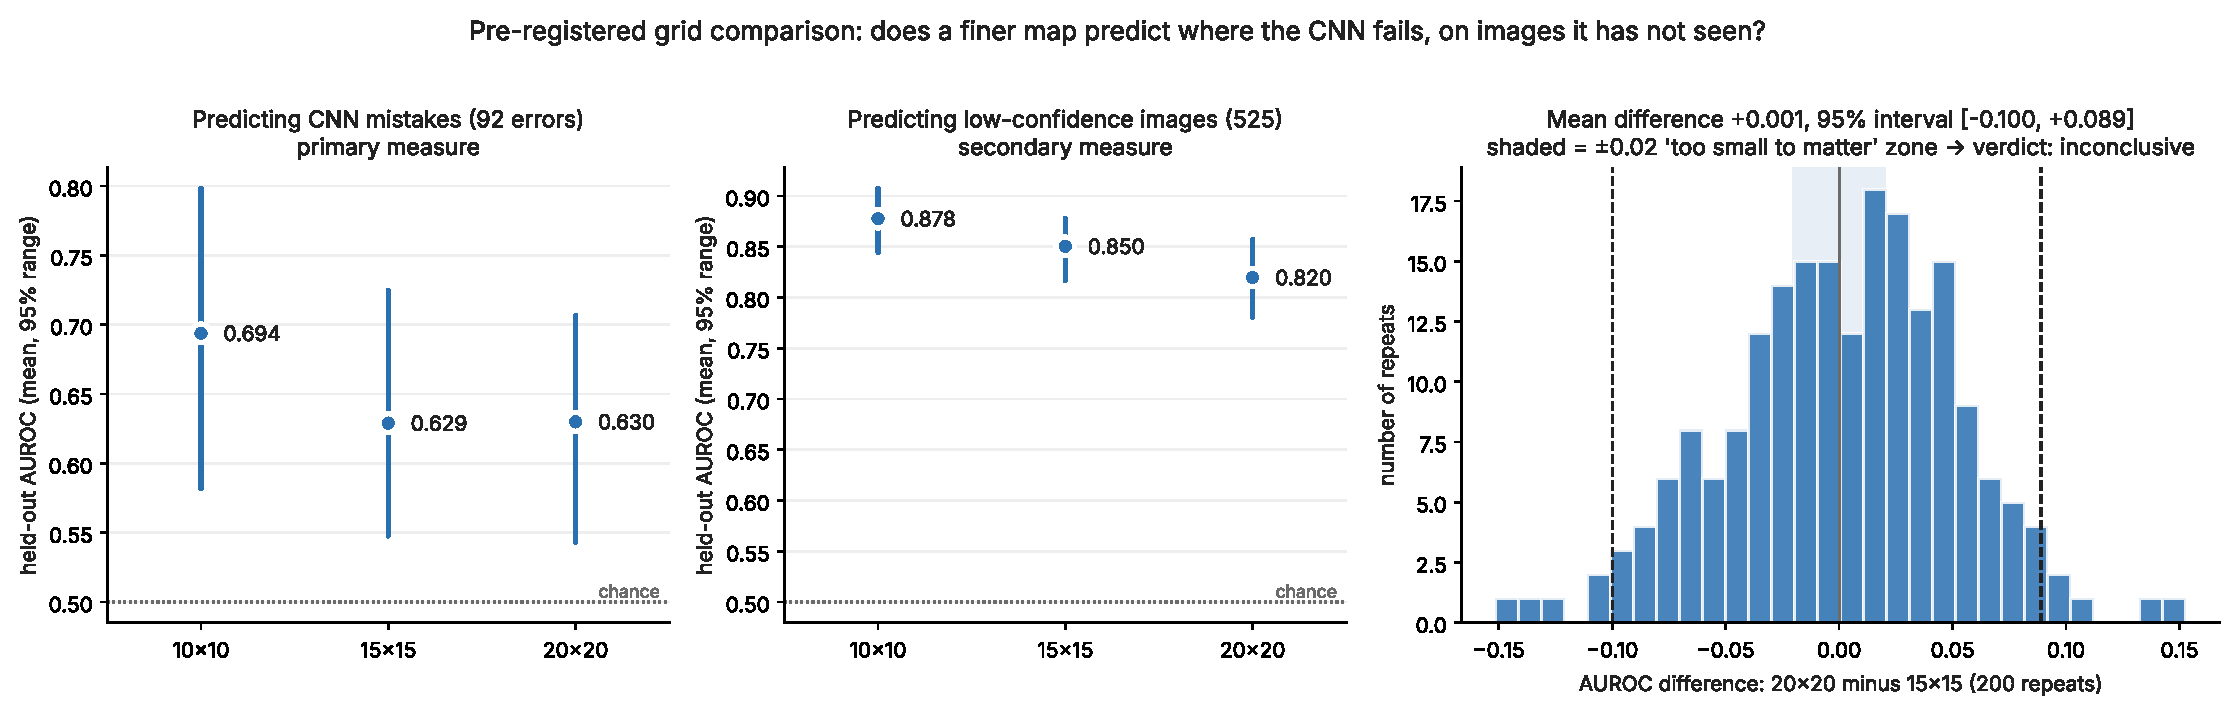
\includegraphics[width=\textwidth]{fig/som_nnsom_training/grid_comparison/grid_comparison_results.pdf}
\caption{Fair grid comparison. Left and middle: held-out AUROC per grid for the CNN's 92 mistakes and for the 525 least-confident images (mean and 95\% range). Right: the 200 differences between 20$\times$20 and 15$\times$15; the range crosses 0 and is wider than the $\pm0.02$ band, so the result is inconclusive.}
\label{fig:gridcmp}
\end{figure}

\begin{figure}[H]
\centering
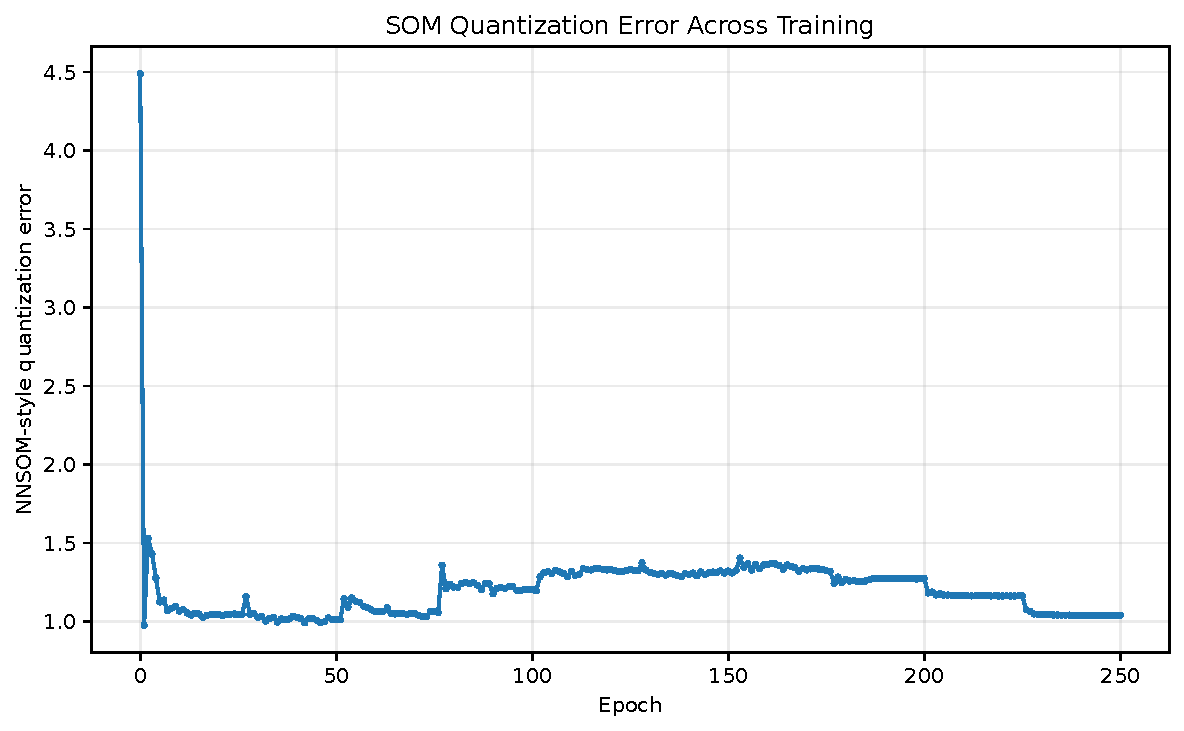
\includegraphics[width=0.62\textwidth]{fig/som_nnsom_training/convergence/som_15x15_nb11_ep250_s42_v2_qe_curve.pdf}
\caption{Quantization error of the 15$\times$15 map on the training images after each of the 250 epochs.}
\label{fig:qe}
\end{figure}

\begin{figure}[H]
\centering
\begin{minipage}[c]{0.48\textwidth}\centering
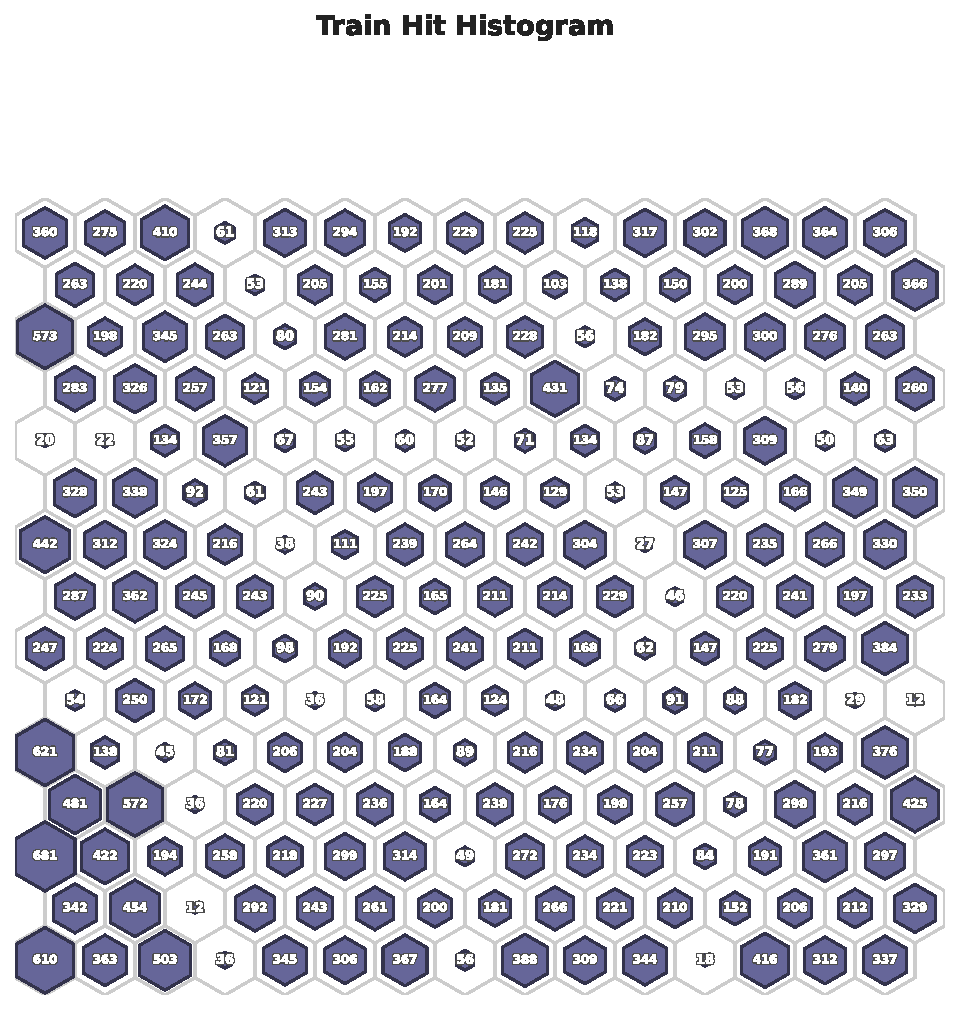
\includegraphics[width=\linewidth,keepaspectratio]{fig/som_nnsom_training/core/train_hit_histogram.pdf}
\end{minipage}\hfill
\begin{minipage}[c]{0.48\textwidth}\centering
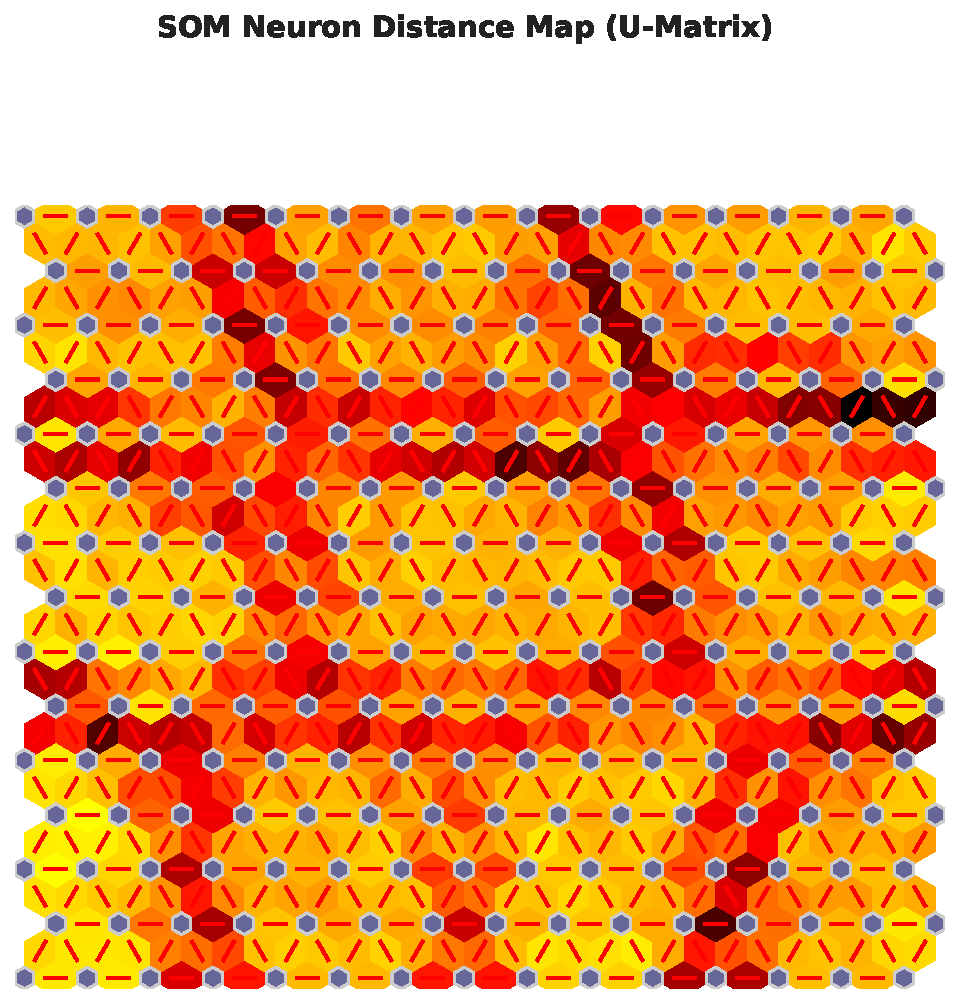
\includegraphics[width=\linewidth,keepaspectratio]{fig/som_nnsom_training/core/u_matrix_neuron_distance.pdf}
\end{minipage}
\caption{Left: hit histogram, the number of training images in each cell (larger hexagon, more images). Right: U-matrix, the distance between neighbouring cells (dark red: a border between groups of cells).}
\label{fig:umatrix}
\end{figure}

\begin{figure}[H]
\centering
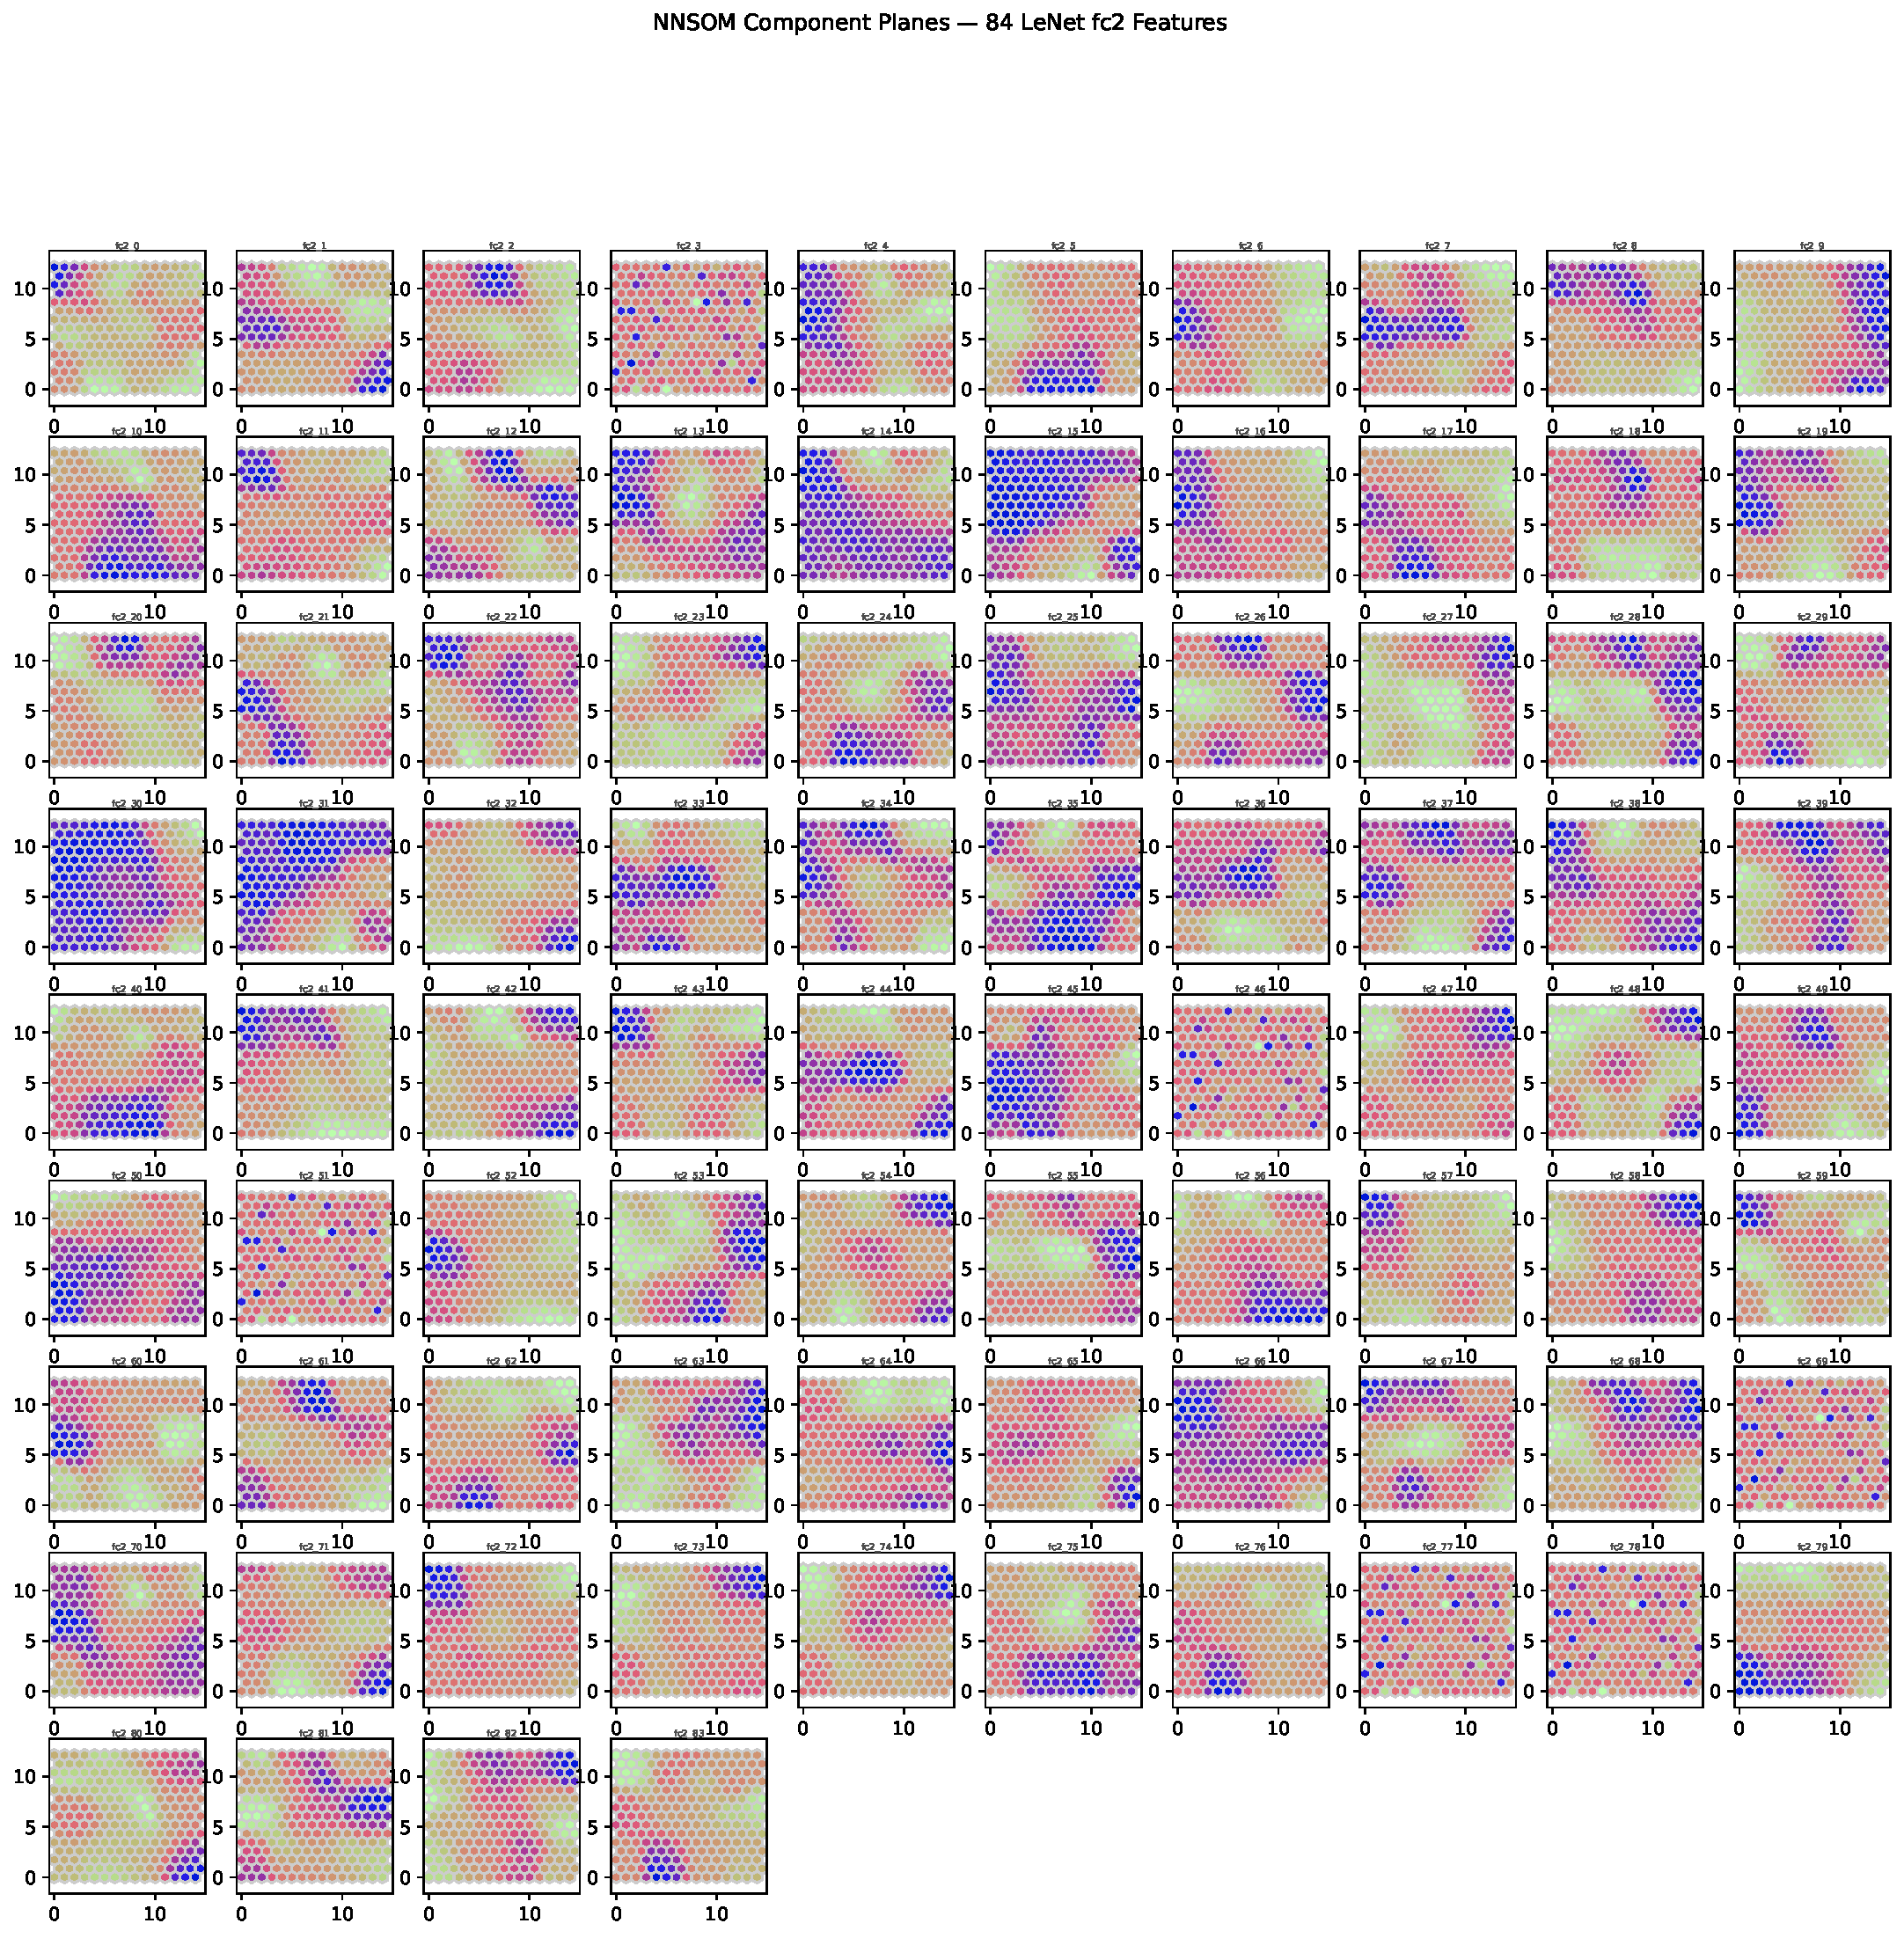
\includegraphics[width=0.80\textwidth]{fig/som_nnsom_training/component_planes/component_planes_all84_nnsom.pdf}
\caption{Component planes of all 84 embedding numbers (one small map each; colour shows where on the grid that number is high or low).}
\label{fig:planes}
\end{figure}

\subsection{Feature-layer ablation}

We also checked the choice of layer, as the proposal asks. We trained SOMs with the same recipe on the earlier layer fc1 (120 numbers) and on fc2, five SOM seeds each, and compared them on rules fixed before the run (Table~\ref{tab:layer_ablation}). The fc2 maps locate the CNN's mistakes clearly better (error-cell AUROC 0.685 against 0.622) and have purer cells, so the choice of fc2 is supported by the data. The fc1 maps separate SVHN slightly better, but by only 0.005 AUROC, far less than the gap to max-softmax and energy. The SOM recipe was tuned on fc2, which may favour it. The fc2 maps of the new seeds also reproduce the main map's values (0.685, 0.982 and 0.981). The fc2 maps also put more of the mistakes in their hotspots; the fc1 maps are slightly better ordered (lower topographic error).

\begin{table}[H]
\centering
\renewcommand{\arraystretch}{1.12}
\small
\begin{tabular}{|l|c|c|c|c|}
\hline
\textbf{Measure (validation images)} & \textbf{fc1} & \textbf{fc2} & \textbf{fc1 $-$ fc2 (95\% interval)} & \textbf{Verdict} \\ \hline
Error-cell AUROC (main) & 0.622 & 0.685 & $-0.062$ ($-0.073$ to $-0.052$) & fc2 better \\ \hline
Weighted purity & 0.961 & 0.982 & $-0.021$ ($-0.022$ to $-0.020$) & fc2 better \\ \hline
QE novelty AUROC (SVHN) & 0.986 & 0.981 & $+0.005$ ($+0.003$ to $+0.006$) & fc1 better \\ \hline
\multicolumn{5}{|l|}{\textit{Also reported (not judged)}} \\ \hline
Hotspot error rate & 0.130 & 0.196 & $-0.065$ ($-0.077$ to $-0.054$) & \\ \hline
Hotspot share of all mistakes & 0.317 & 0.376 & $-0.059$ ($-0.085$ to $-0.032$) & \\ \hline
Topographic error TE1 (\%) & 5.45 & 6.35 & $-0.90$ ($-1.07$ to $-0.74$) & \\ \hline
\end{tabular}
\caption{Feature-layer ablation: SOMs on the 120-number layer fc1 and the 84-number layer fc2 of the same network, same recipe, mean over 5 SOM seeds each. Statements and rules fixed before the run.}
\label{tab:layer_ablation}
\end{table}

\section{Cluster Analysis}\label{sec:cluster}

\begin{itemize}[leftmargin=1.4em, itemsep=2pt]
\item \textbf{Method.} Each training and validation image is assigned to its best-matching cell. For every cell we count the images of each digit (the class--cell intersection, computed with NNSOM's \texttt{cal\_class\_cluster\_intersect}), and from these counts the cell's most common digit, its purity and its entropy \cite{vesanto2000clustering}. To see whether the purity is more than chance, we shuffle the digit labels 1,000 times, keep every image in its cell, and compute the purity again.

\item \textbf{The digits form clean regions (Figure~\ref{fig:classmap}).} Each digit occupies its own region of the map, with 15 to 29 cells per digit. On validation images the purity is 98.19\% (training: 98.94\%), against 17.4\% (95\% range 17.0--17.7\%) with shuffled labels ($p=0.001$). 154 of the 225 cells hold only one digit.

\item \textbf{Mixed cells sit on borders.} 44 cells have a purity below 95\%, and 25 below 80\% (the lowest is 44\%). In the purity map these cells lie on the borders between digit regions, the same places where the U-matrix shows high distances. This is where the CNN's embeddings of two digits come close.

\item \textbf{Where confusions happen (Figure~\ref{fig:overlay}).} The three most frequent validation confusions (4 called 9, 5 called 0 and 9 called 4, six times each) each fall on only four or five cells, mostly cells of the digit they were mistaken for. A confused image therefore tends to sit inside the region of the wrong digit, which is why the CNN calls it that digit.
\end{itemize}

\begin{figure}[H]
\centering
\begin{minipage}[c]{0.46\textwidth}\centering
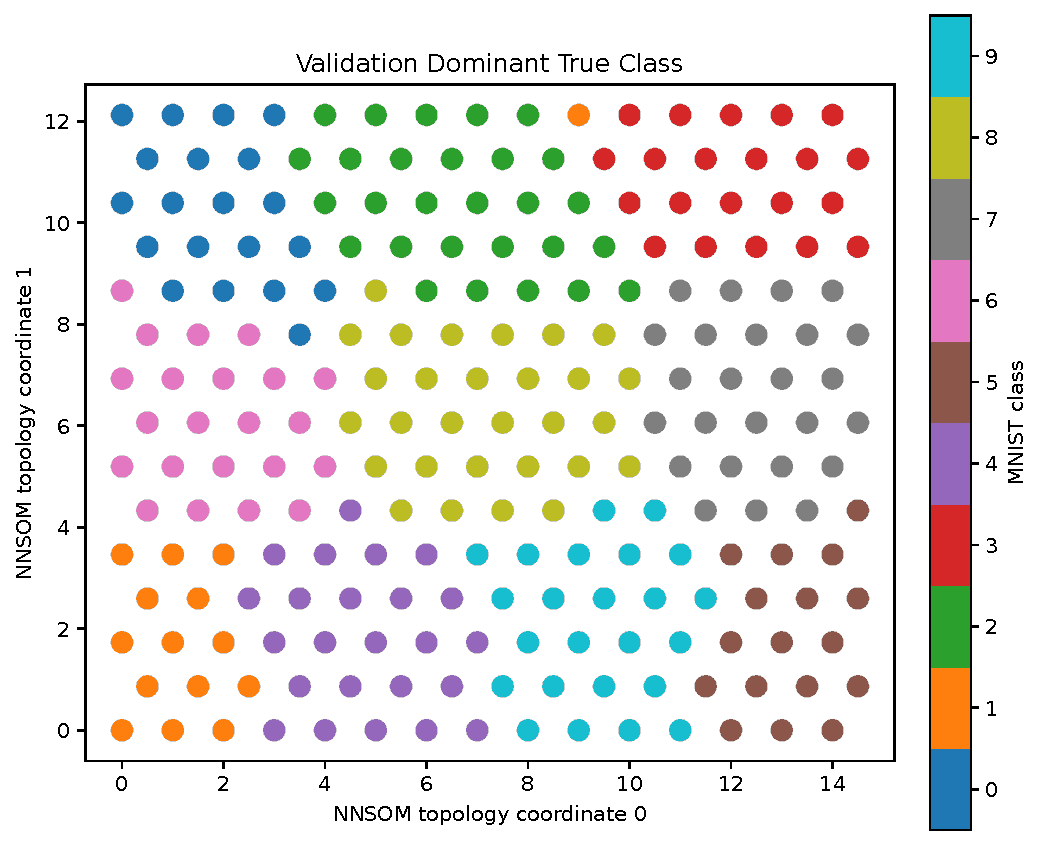
\includegraphics[width=\linewidth,keepaspectratio]{fig/cluster_analysis/analysis_maps/validation_dominant_class.pdf}
\end{minipage}\hfill
\begin{minipage}[c]{0.52\textwidth}\centering
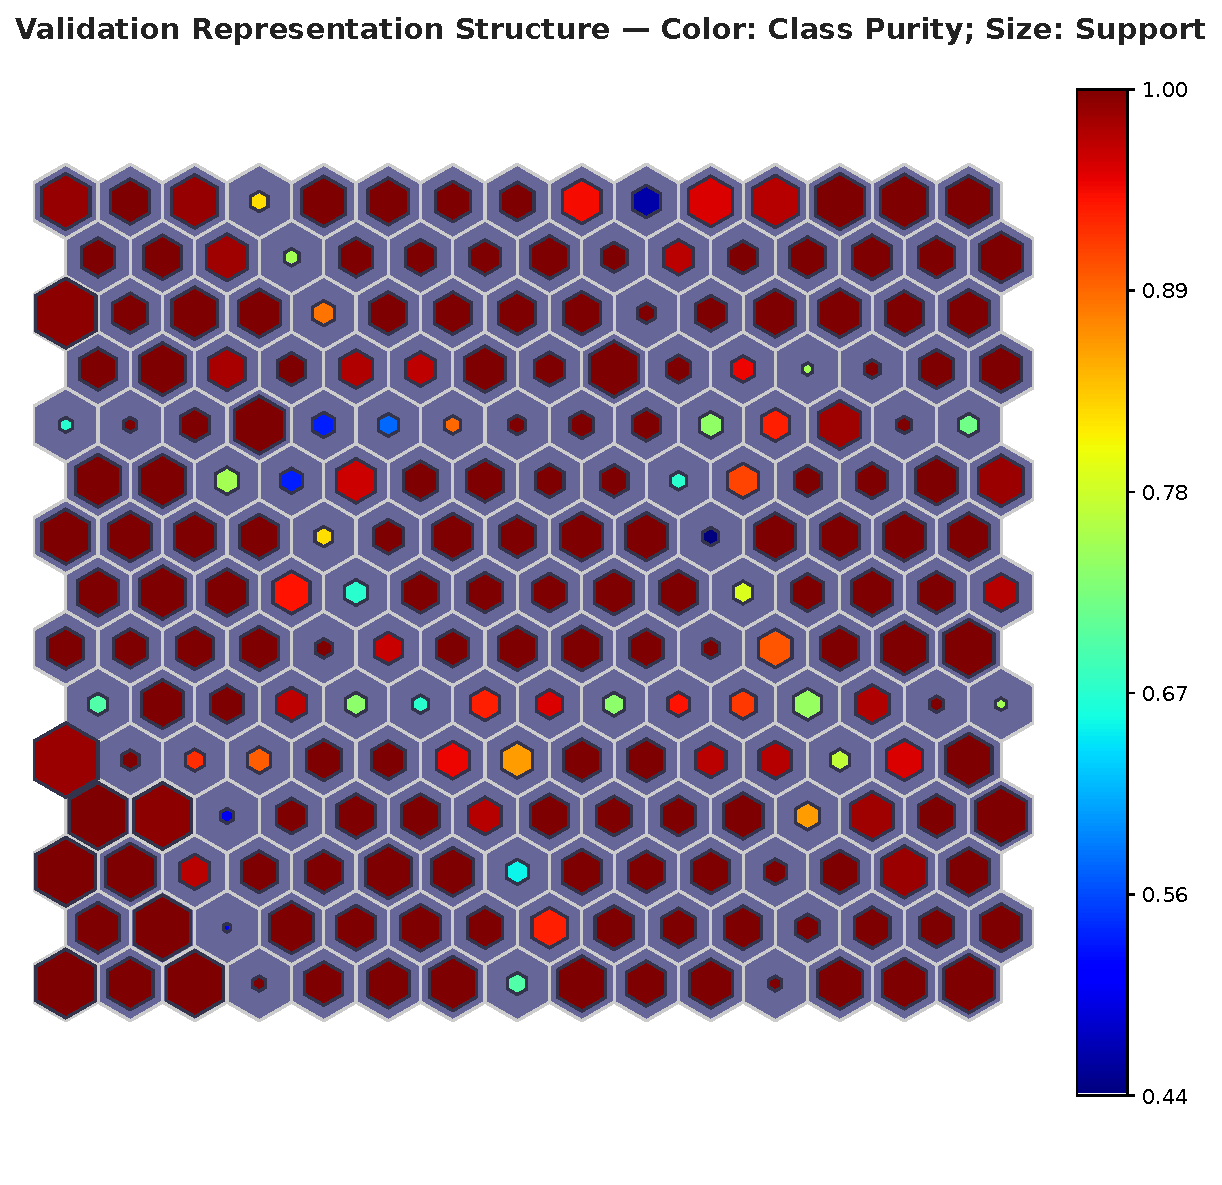
\includegraphics[width=\linewidth,keepaspectratio]{fig/cluster_analysis/analysis_maps/validation_purity_support.pdf}
\end{minipage}
\caption{Left: the most common digit of each cell (validation images). Right: purity of each cell (colour) and number of validation images in it (size). Low-purity cells lie on the borders between digit regions.}
\label{fig:classmap}
\end{figure}

\begin{figure}[H]
\centering
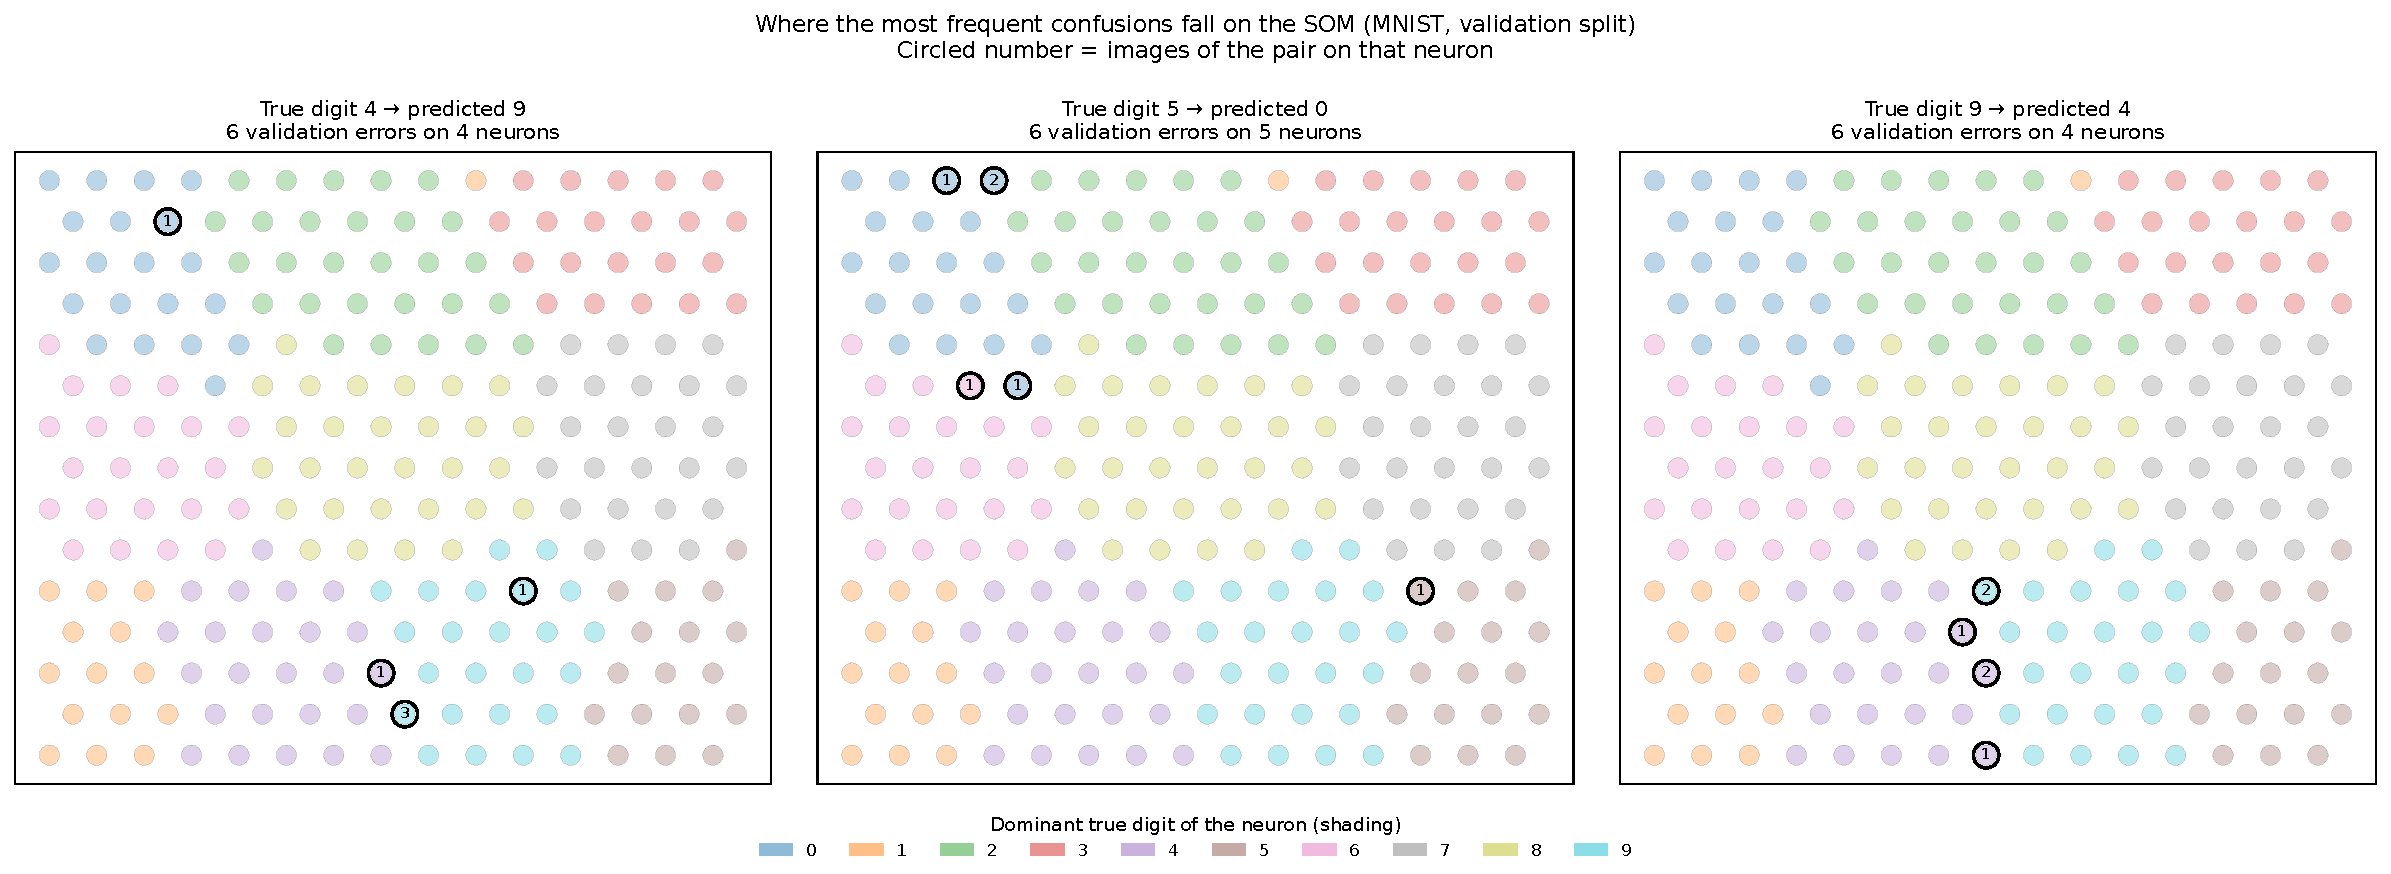
\includegraphics[width=\textwidth]{fig/cluster_analysis/analysis_maps/validation_confusion_overlay.pdf}
\caption{Where the three most frequent confusions fall on the map (validation images). Circled cells hold images of that confusion; the number is how many.}
\label{fig:overlay}
\end{figure}

\section{Error Pattern Analysis}\label{sec:error}

\begin{itemize}[leftmargin=1.4em, itemsep=2pt]
\item \textbf{Correct against wrong.} The CNN gets 92 of the 10,500 validation images wrong (0.88\%). It is less sure when it is wrong (average confidence 0.833) than when it is right (0.997). Wrong images also sit farther from their cell (average distance 1.349, against 0.960 for correct images).

\item \textbf{Hotspots.} We rank the cells by the lower end of the 95\% Wilson interval of their error rate, and call the top 5\% of the cells (11 cells) hotspots. On the full validation set these 11 cells hold 1.7\% of the images but 37\% of the mistakes (34 of 92). That number is too high, because the same images were used to pick the hotspots and to count their mistakes. The fair test picks the hotspots on a random half of the validation images and counts the mistakes on the other half, 200 times. It gives a concentration ratio of 11.1 (95\% range 6.1--17.6), against about 0.94 when the mistake labels are shuffled ($p=0.005$, Table~\ref{tab:hotspots}).

\item \textbf{Overlap regions.} A cell's error rate goes down as its purity goes up (Spearman $-0.810$) and goes up as its digit mix grows ($+0.816$), far beyond chance ($p=0.005$). So the mistakes sit where digits overlap. Both findings hold on the 10$\times$10 and 20$\times$20 maps as well (Table~\ref{tab:hotspots}); the rules for this check were written down before it was run.

\item \textbf{Error maps (Figure~\ref{fig:errormaps}).} Most cells make no mistakes at all. The hotspots are scattered small cells, mostly on the borders between digit regions, not one large bad area.

\item \textbf{The images in the hotspots (Figure~\ref{fig:samples}), and why they are hard.} We looked at one misclassified image from each hotspot. Our reading, which is a hypothesis and not a tested result:
  \begin{itemize}[leftmargin=1.2em, itemsep=0pt]
  \item \emph{Digits that share strokes:} a 9 with an open loop read as 4, a 7 with a crossbar read as 2, or a 5 with a closed lower curve read as 6, 8 or 0.
  \item \emph{Unusual handwriting:} very slanted 1s, a 7 written like a 3, and one blot-like 2 read as 0.
  \item \emph{Not noise:} the CNN is often still very sure of the wrong answer (confidence above 0.97 in three of the eleven examples), so these images look like the wrong digit to the network, not like random noise.
  \end{itemize}

\item \textbf{Comparison with simple baselines (Table~\ref{tab:baselines}).} Because the SOM is trained on the CNN's own embeddings, we checked whether simpler tools find the same pattern. A k-means grouping with 225 groups finds mistakes as well as the SOM cells do (AUROC 0.693 against 0.685, overlapping ranges). The impurity of the 15 nearest training embeddings does much better (0.874), and the CNN's own confidence (maximum softmax probability \cite{hendrycks2017baseline}) does best (0.981). When every method may flag the same 1.6\% of the images as the SOM's hotspots, the SOM catches 18\% of the mistakes, nearest-neighbour impurity 49\% and the confidence score 53\%. These baseline checks were added after the main results and are exploratory.
\end{itemize}

\begin{table}[H]
\centering
\renewcommand{\arraystretch}{1.12}
\small
\begin{tabular}{|l|c|c|c|}
\hline
\textbf{Measure (validation images)} & \textbf{10$\times$10} & \textbf{15$\times$15} & \textbf{20$\times$20} \\ \hline
Hotspot cells & 5 & 11 & 20 \\ \hline
Concentration ratio (95\% range) & 10.5 (5.4--17.3) & 11.1 (6.1--17.6) & 13.4 (8.0--19.3) \\ \hline
Chance level (median) & 0.98 & 0.94 & 0.93 \\ \hline
Spearman, error rate vs.\ purity & $-0.755$ & $-0.810$ & $-0.766$ \\ \hline
Spearman, error rate vs.\ digit mix (entropy) & $+0.778$ & $+0.816$ & $+0.768$ \\ \hline
Distance to cell, wrong / correct images & 1.481 / 1.078 & 1.349 / 0.960 & 1.279 / 0.895 \\ \hline
\end{tabular}
\caption{Where the 92 validation mistakes gather, on three grid sizes. Hotspots are picked on one half of the validation images and measured on the other (200 splits); chance comes from 200 shuffles of the mistake labels. All $p=0.005$, the smallest value possible with 200 shuffles. The ratios should not be used to compare grids with each other, because the grids have different numbers of hotspots.}
\label{tab:hotspots}
\end{table}

\begin{table}[H]
\centering
\renewcommand{\arraystretch}{1.12}
\footnotesize\setlength{\tabcolsep}{3pt}
\begin{tabular}{|l|c|c|c|c|}
\hline
\textbf{Method} & \textbf{AUROC (95\% range)} & \textbf{Hotspot ratio} & \textbf{Images flagged} & \textbf{Mistakes caught} \\ \hline
SOM cell (15$\times$15) & 0.685 (0.624--0.738) & 11.1 (6.1--17.6) & 1.6\% & 18.1\% \\ \hline
k-means cell (225) & 0.693 (0.651--0.729) & 5.6 (4.6--6.1) & 3.8\% & 20.4\% \\ \hline
15-nearest-neighbour impurity & 0.874 (0.829--0.917) & -- & 1.6\% & 48.7\% \\ \hline
Max-softmax confidence & 0.981 (0.974--0.987) & -- & 1.6\% & 53.3\% \\ \hline
\end{tabular}
\caption{How well each score finds the 92 validation mistakes. For the last two rows the images flagged are set to the SOM's 1.6\% so that the comparison is fair (95\% ranges: 39.6--58.3\% and 44.5--64.3\%). Exploratory.}
\label{tab:baselines}
\end{table}

\begin{figure}[H]
\centering
\begin{minipage}[c]{0.52\textwidth}\centering
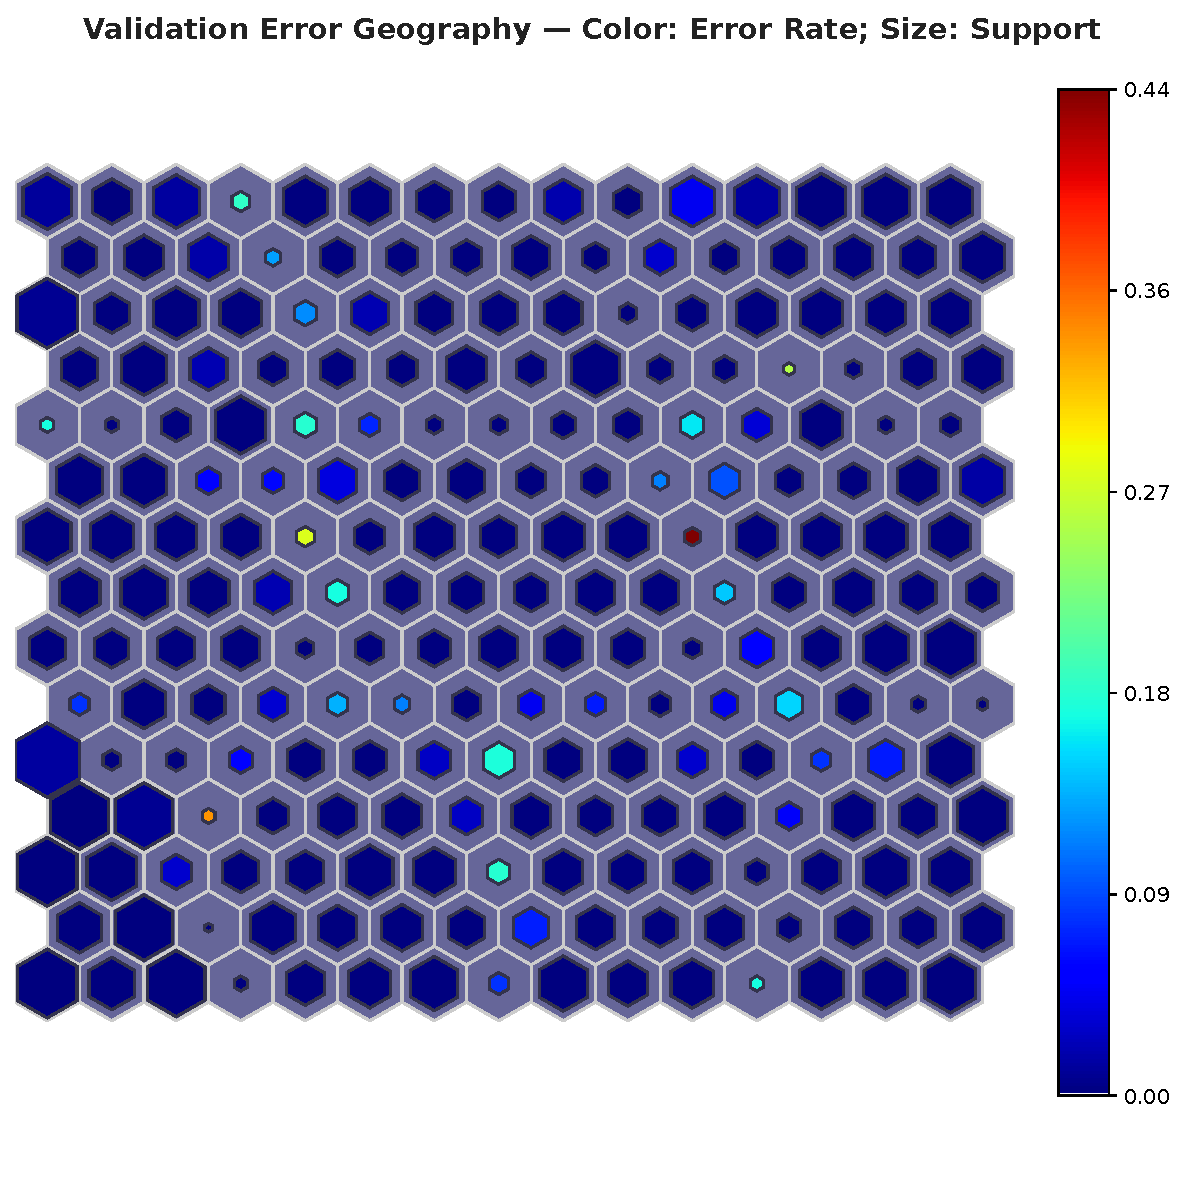
\includegraphics[width=\linewidth,keepaspectratio]{fig/error_pattern_analysis/analysis_maps/validation_error_rate_support.pdf}
\end{minipage}\hfill
\begin{minipage}[c]{0.46\textwidth}\centering
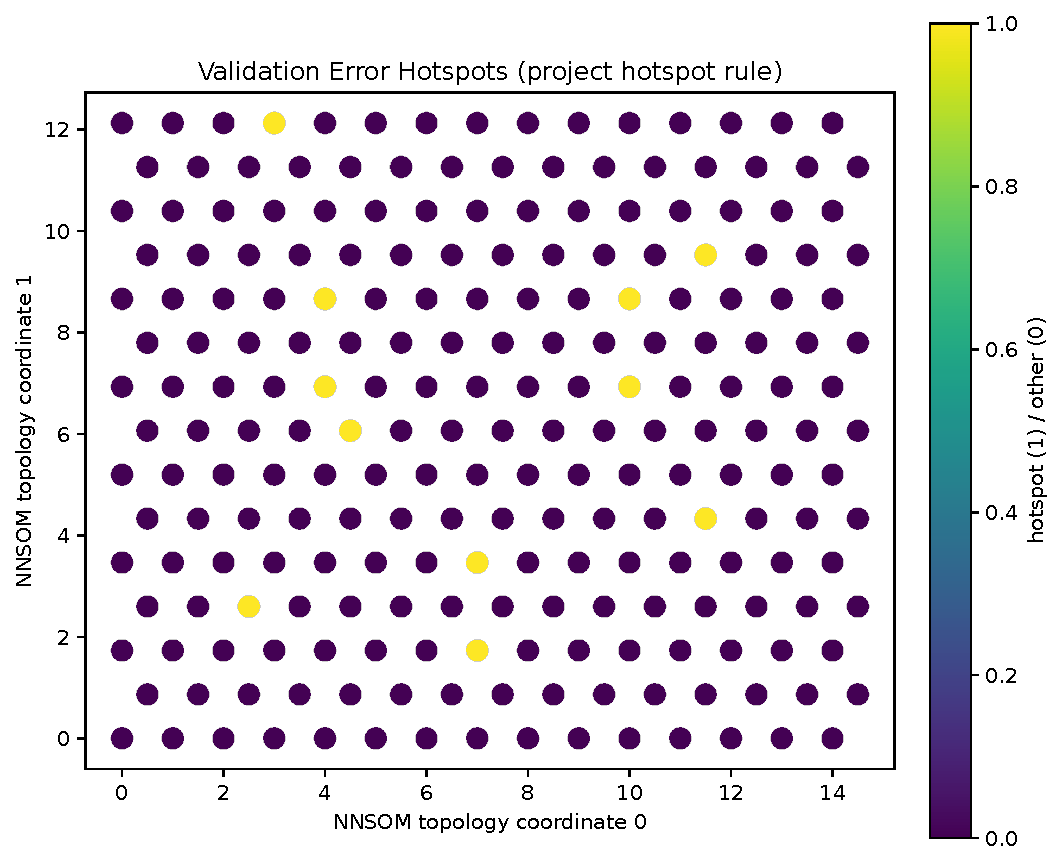
\includegraphics[width=\linewidth,keepaspectratio]{fig/error_pattern_analysis/analysis_maps/validation_hotspot_map.pdf}
\end{minipage}\\[4pt]
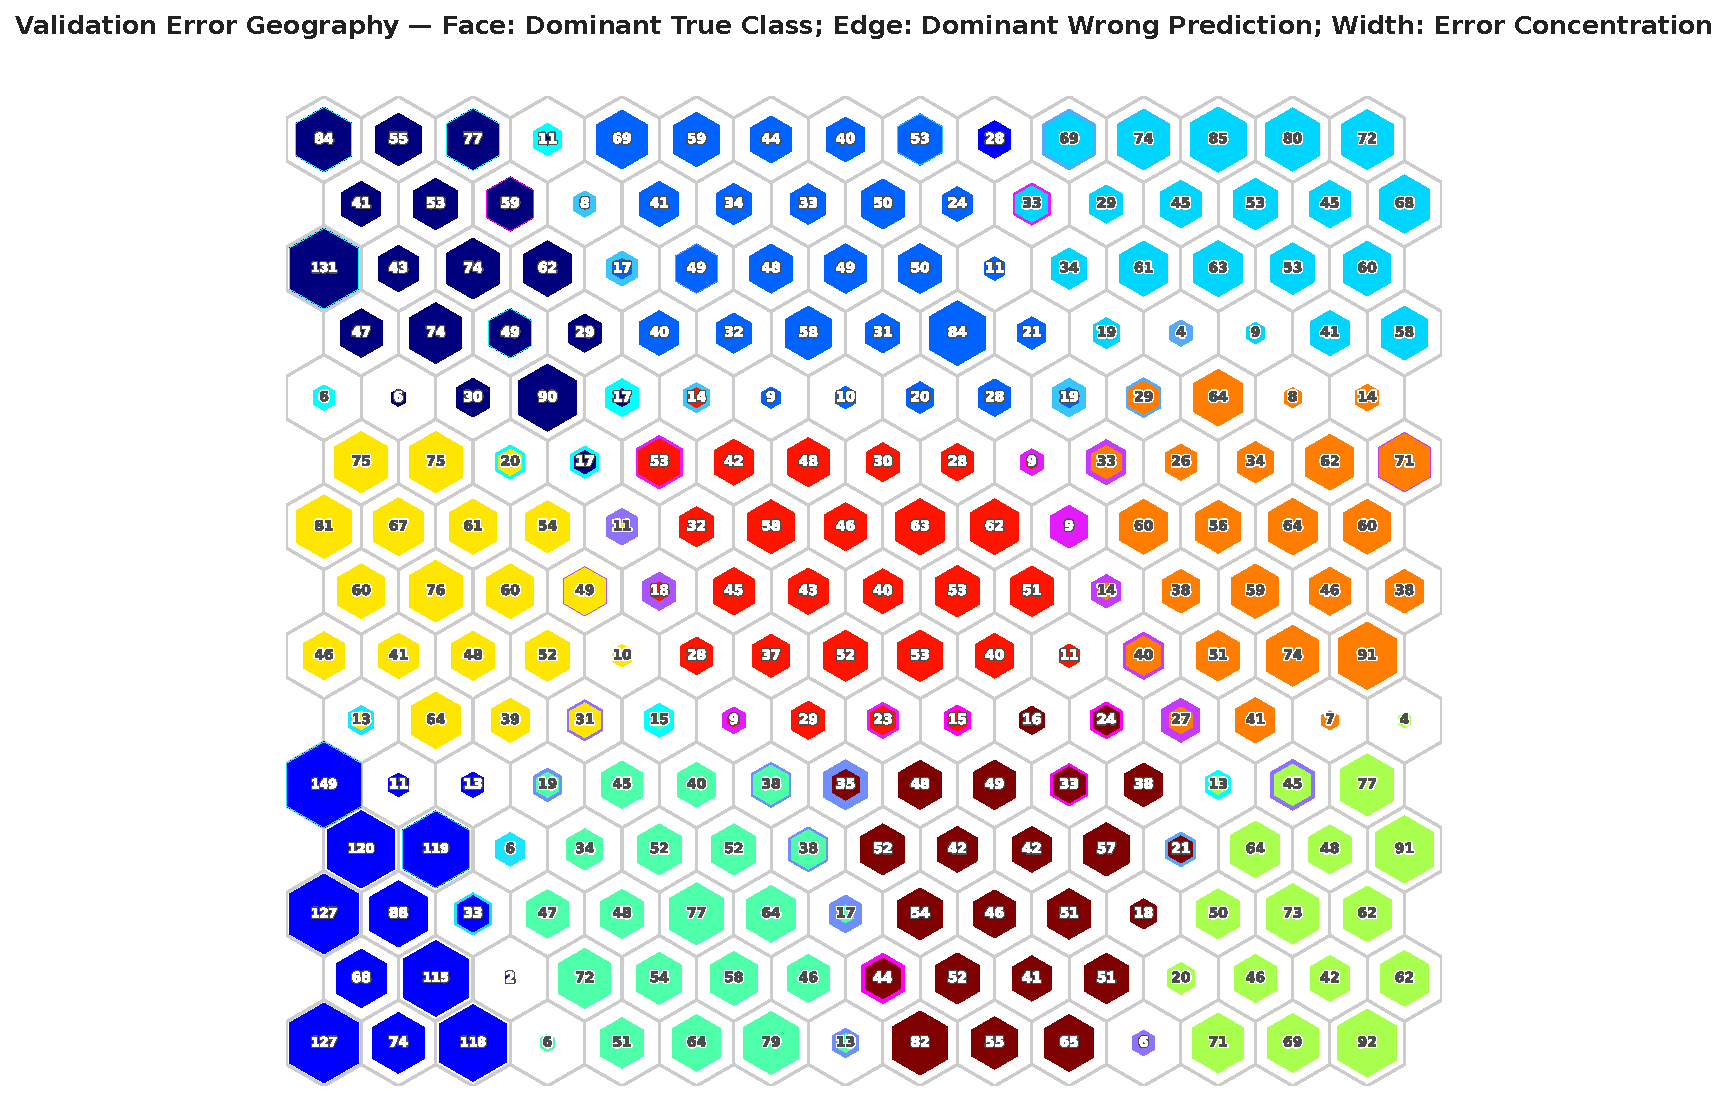
\includegraphics[width=0.62\textwidth,keepaspectratio]{fig/error_pattern_analysis/analysis_maps/validation_complex_error_map.pdf}
\caption{Top left: error rate of each cell (colour) and number of validation images (size). Top right: the 11 hotspot cells (yellow). Bottom: error map, where the fill is the cell's most common true digit, the edge colour its most common wrong answer, and the edge width how many mistakes it holds.}
\label{fig:errormaps}
\end{figure}

\begin{figure}[H]
\centering
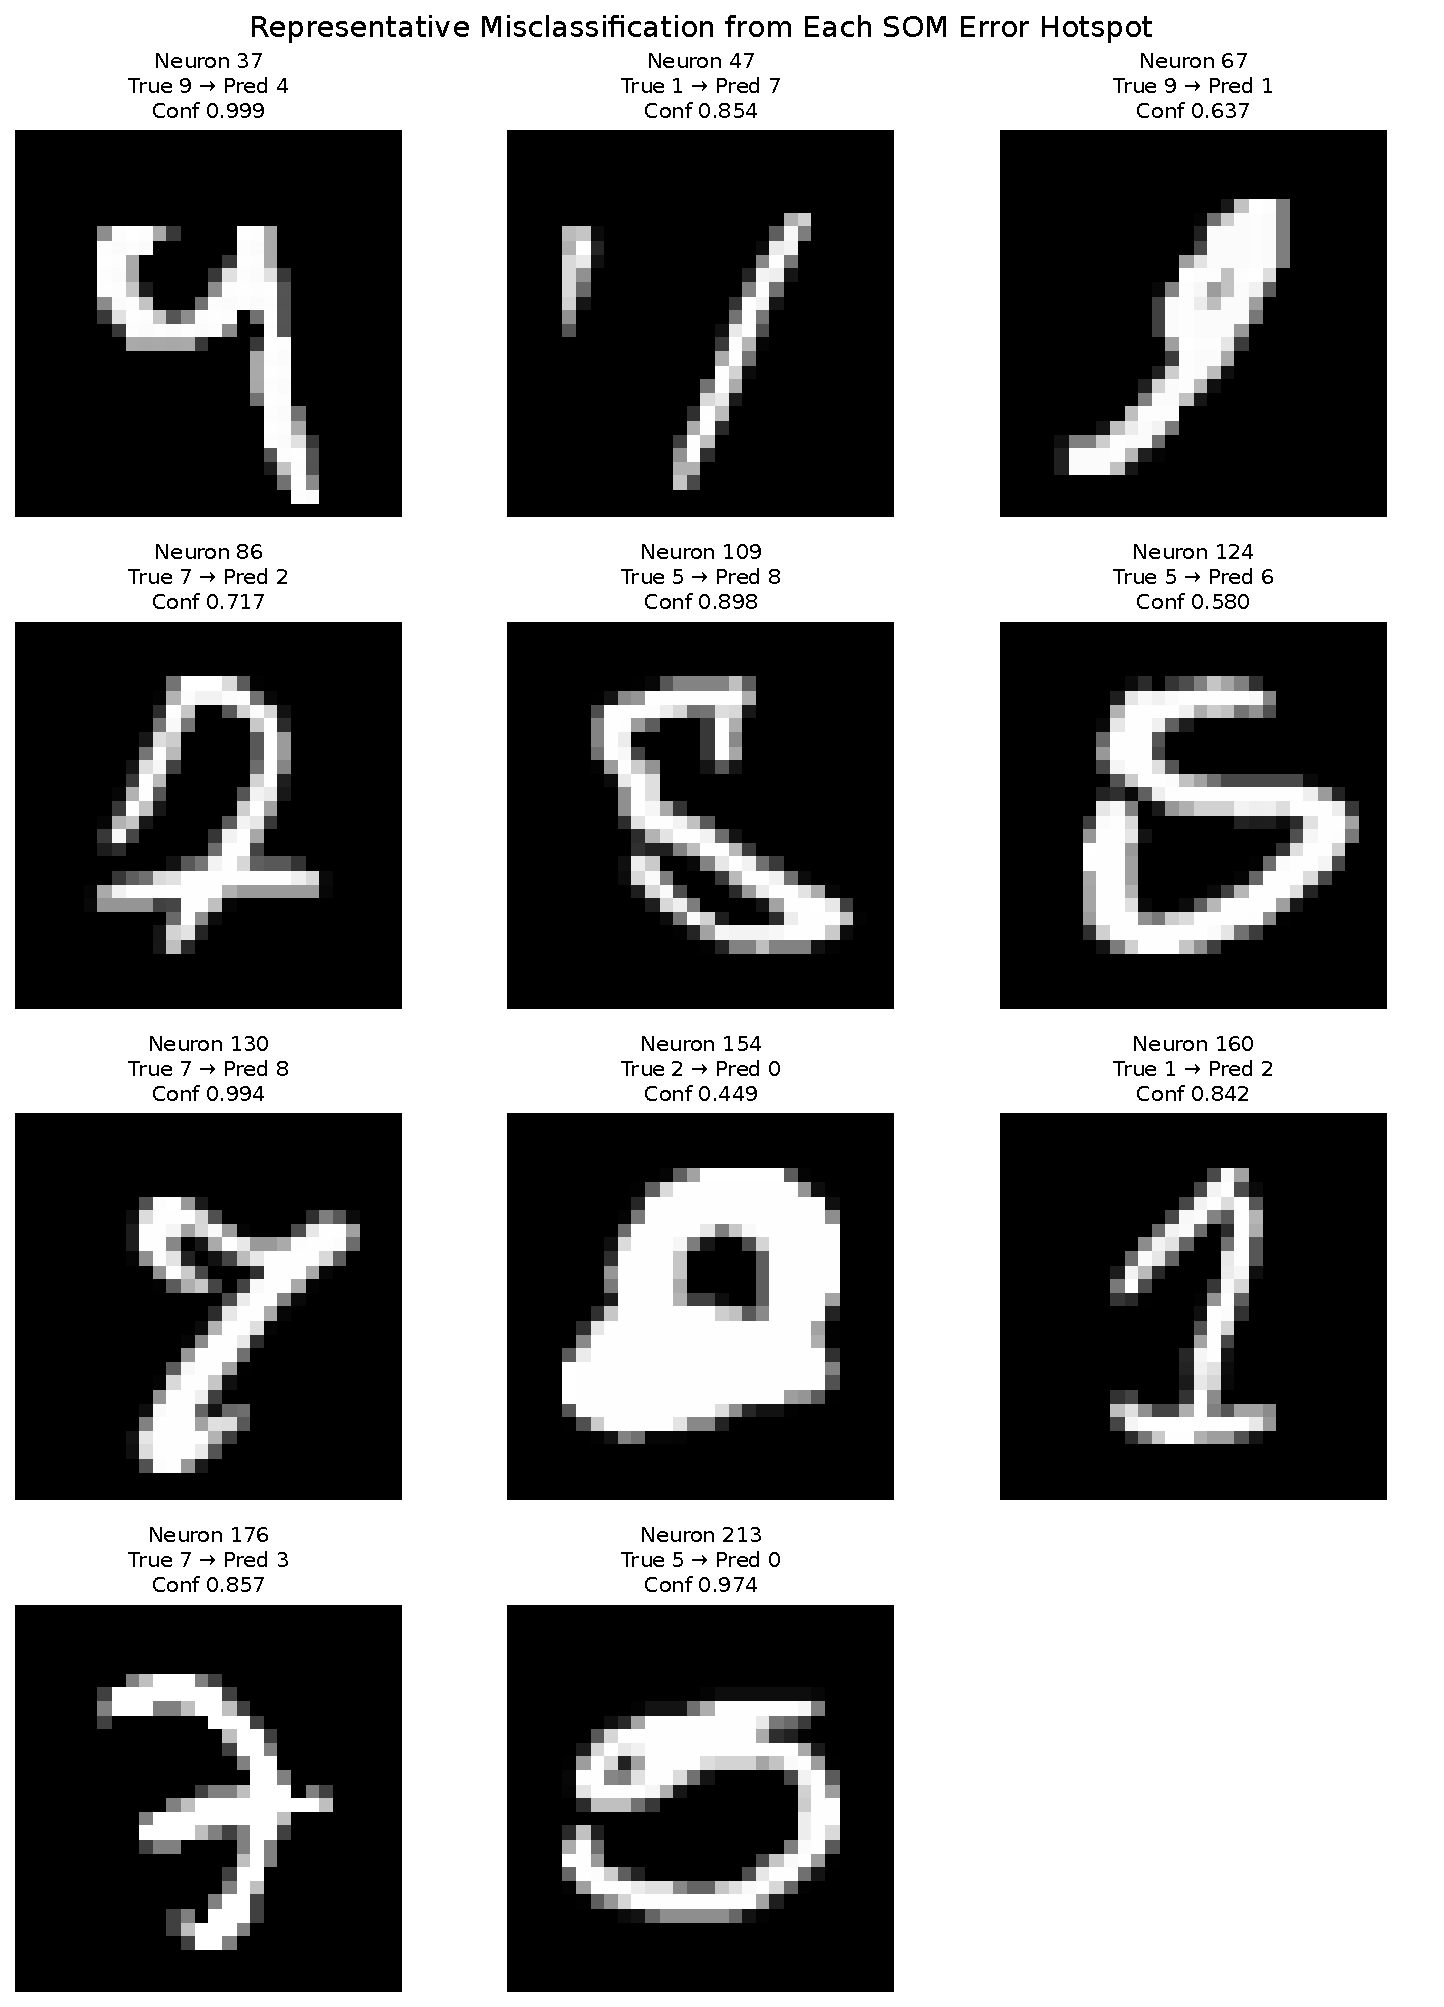
\includegraphics[width=0.62\textwidth,keepaspectratio]{fig/error_pattern_analysis/representative_samples/hotspot_representatives.pdf}
\caption{One misclassified validation image from each of the 11 hotspot cells, with the true digit, the CNN's answer and its confidence.}
\label{fig:samples}
\end{figure}

\section{Leakage Control}

The SOM work uses the training and validation splits only:
\begin{itemize}
    \item The SOM was trained on the 49,000 training embeddings. The scaler that
    maps the embeddings to $[-1,1]$ was fitted on the training embeddings only and
    then applied unchanged to the validation embeddings.
    \item SOM settings were compared on validation data only (the configuration
    sets \texttt{use\_test\_for\_selection: false}). The grid comparison and the
    error-pattern check on other grids followed rules written down before they were run;
    the selection history of the grid size is recorded in the project's deviation log.
    \item The maps, purity, label-shuffle control and error maps in this report
    use validation images. The test embeddings are never loaded: the model's
    metrics file records that the test split was not evaluated, and the analysis
    code refuses to run otherwise.
    \item The CNN that produced the embeddings used the same validation split to
    choose its checkpoint, so validation is not entirely untouched by model
    development; the test split remains unused for the final evaluation.
\end{itemize}

\section{Deviations from the plan}

\begin{itemize}[leftmargin=1.4em, itemsep=2pt]
\item \textbf{Test images not mapped.} The plan says to assign the training and test images to their cells. We map the training and validation images only, so that the test split stays untouched until the final evaluation.
\item \textbf{Grid size.} An earlier selection rule picked 20$\times$20, but its runs were later retrained under the same run names, and on the new files the same rule picks 10$\times$10. Both outcomes are kept in the deviation log. We then ran the fair comparison of Table~\ref{tab:grids}, which could not separate the grids, and use 15$\times$15 as the main map with 10$\times$10 and 20$\times$20 as checks.
\item \textbf{No learning rate.} NNSOM's batch rule has no learning rate, so only the grid size, the starting neighbourhood radius and the number of epochs were set.
\end{itemize}

\section{Discussion}
\begin{itemize}[leftmargin=1.4em, itemsep=2pt]
\item \textbf{The map is a good picture of what the CNN has learned.} The digits form clean, separate regions far beyond chance, and the borders between them are clearly visible in the U-matrix and the purity map.
\item \textbf{The CNN's mistakes are not random.} They gather in a few small cells on the borders between digits that look alike, and this holds on three grid sizes and against chance. The hotspot images suggest two kinds of hard cases: digits that share strokes, and unusual handwriting.
\item \textbf{The SOM explains, it does not detect best.} A plain k-means grouping finds mistakes as well as the SOM cells, and the CNN's own confidence does much better. So the value of the SOM is in showing \emph{where} the mistakes are and which digits they involve, not in flagging them.
\item \textbf{Limits.} There are only 92 validation mistakes, so the intervals are wide and differences below about 0.1 AUROC cannot be seen. MNIST is easy, so harder data are needed before general conclusions. The hotspot explanations come from looking at a few images and are hypotheses.
\end{itemize}

\section{Conclusion and Next Phase}

\begin{itemize}[leftmargin=1.4em, itemsep=2pt]
\item A 15$\times$15 SOM trained on the CNN's 84-number embeddings orders the MNIST digits into clean regions, with 98.2\% purity on validation images.
\item The CNN's 92 validation mistakes gather in 11 hotspot cells (about 11 times their fair share) where digits overlap, and the finding holds on 10$\times$10 and 20$\times$20 maps.
\item Simple baselines find mistakes as well (k-means) or better (nearest neighbours, CNN confidence), so we use the SOM as a map of where the CNN fails.
\item \textbf{Next phase.} Phase 3 uses the same frozen map to test whether an image far from its cell (large quantization error) is unlike the training data; the larger distance of misclassified images (1.349 against 0.960) is a first hint. Phase 4 uses the hotspot cells to choose images for retraining.
\end{itemize}

\printbibliography[title={References}]

\end{document}
